\begin{enumerate}[label=\thesubsection.\arabic*,ref=\thesubsection.\theenumi]
\item 
Find the area between the curves $y=x$ and $y=x^2$.
\\
\solution
\label{chapters/12/8/3/2}
	\begin{figure}[H]
		\centering
 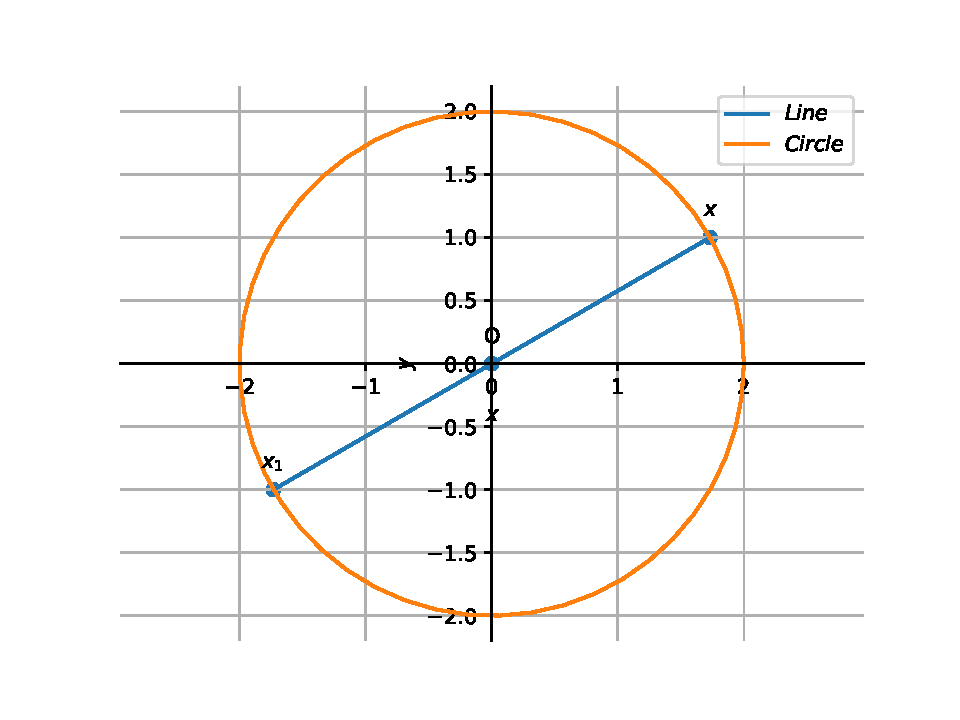
\includegraphics[width=0.75\columnwidth]{chapters/12/8/1/6/figs/conics-fig.pdf} 
		\caption{}
		\label{fig:12/8/1/6}
  	\end{figure}
  From the given information, the parameters of the  circle and line are
                      \begin{align}
			      f= -4, \vec{u}=\vec{0}, \vec{V}=\vec{I}, \vec{m}=\myvec{1 \\ \sqrt{3}}, \vec{h} = \vec{0}
		\label{eq:12/8/1/6}
                    \end{align}                                                                              
Substituting		    the above parameters in  
\eqref{eq:tangent_roots},
	  \begin{align}                                                                               
		  \mu= \sqrt{3}
	  \end{align}
	  yielding  
the desired point of intersection as                                               
\begin{align}
	\vec{x} = \myvec{\sqrt{3} \\ 1}                               
\end{align}
Note that we have chosen only the point of intersection in the first quadrant as shown in 
		\figref{fig:12/8/1/6}.
From
		\eqref{eq:12/8/1/6},
		the angle between the given line and the x axis is
\begin{align}
	\theta=30\degree
\end{align} 
and
the area of the sector is 
\begin{align}
	{\frac{\theta}{360}}\pi r^2=
	\frac{\pi}{3}
\end{align}

\item 
Find the area of the region bounded by the curve $y^2=x$ and the lines $x=1$ and $x=4$ and the axis in the first quadrant.
\label{chapters/12/8/1/1}
	\\
	\solution
	\begin{figure}[H]
		\centering
 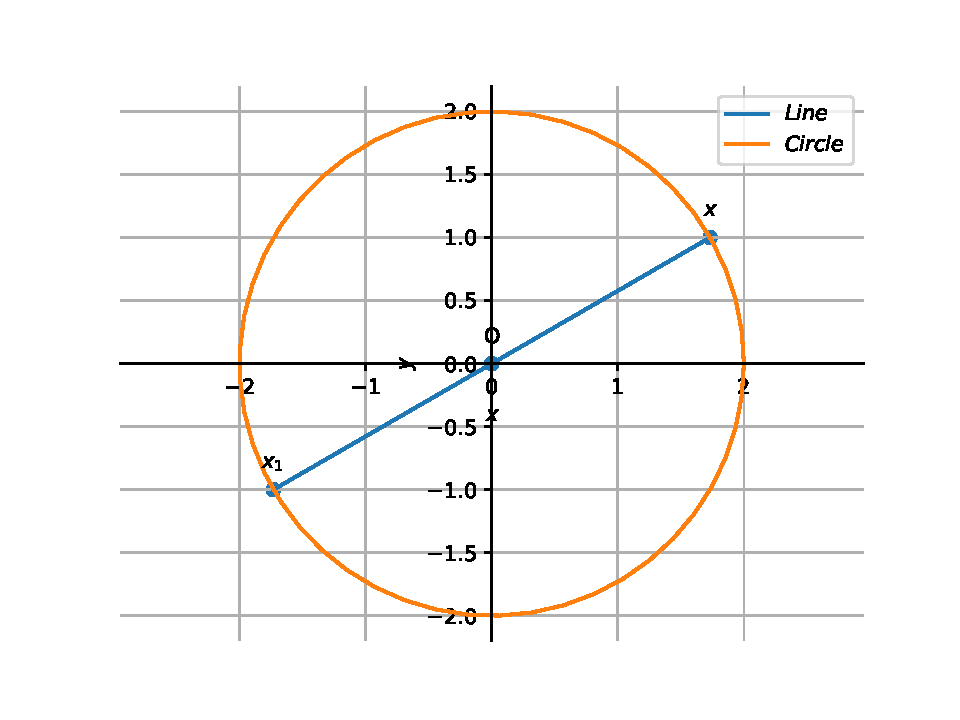
\includegraphics[width=0.75\columnwidth]{chapters/12/8/1/6/figs/conics-fig.pdf} 
		\caption{}
		\label{fig:12/8/1/6}
  	\end{figure}
  From the given information, the parameters of the  circle and line are
                      \begin{align}
			      f= -4, \vec{u}=\vec{0}, \vec{V}=\vec{I}, \vec{m}=\myvec{1 \\ \sqrt{3}}, \vec{h} = \vec{0}
		\label{eq:12/8/1/6}
                    \end{align}                                                                              
Substituting		    the above parameters in  
\eqref{eq:tangent_roots},
	  \begin{align}                                                                               
		  \mu= \sqrt{3}
	  \end{align}
	  yielding  
the desired point of intersection as                                               
\begin{align}
	\vec{x} = \myvec{\sqrt{3} \\ 1}                               
\end{align}
Note that we have chosen only the point of intersection in the first quadrant as shown in 
		\figref{fig:12/8/1/6}.
From
		\eqref{eq:12/8/1/6},
		the angle between the given line and the x axis is
\begin{align}
	\theta=30\degree
\end{align} 
and
the area of the sector is 
\begin{align}
	{\frac{\theta}{360}}\pi r^2=
	\frac{\pi}{3}
\end{align}

\item 
Find the area of the region bounded by the curve $y^2=9x$ and the lines $x=2$ and $x=4$ and the axis in the first quadrant.
\\
\solution
\label{chapters/12/8/1/2}
	\begin{figure}[H]
		\centering
 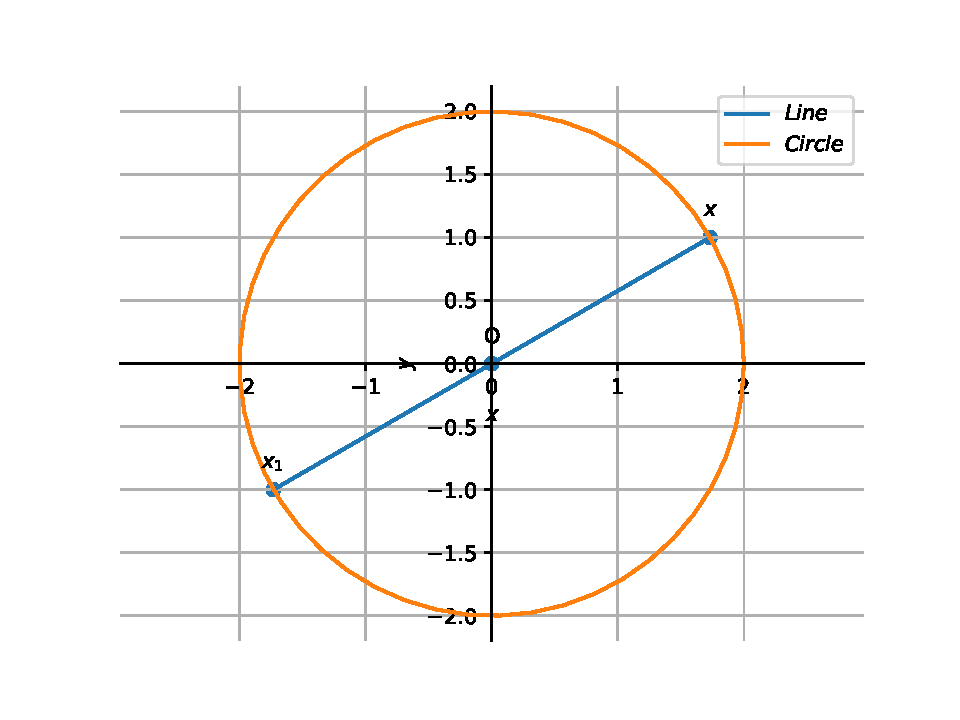
\includegraphics[width=0.75\columnwidth]{chapters/12/8/1/6/figs/conics-fig.pdf} 
		\caption{}
		\label{fig:12/8/1/6}
  	\end{figure}
  From the given information, the parameters of the  circle and line are
                      \begin{align}
			      f= -4, \vec{u}=\vec{0}, \vec{V}=\vec{I}, \vec{m}=\myvec{1 \\ \sqrt{3}}, \vec{h} = \vec{0}
		\label{eq:12/8/1/6}
                    \end{align}                                                                              
Substituting		    the above parameters in  
\eqref{eq:tangent_roots},
	  \begin{align}                                                                               
		  \mu= \sqrt{3}
	  \end{align}
	  yielding  
the desired point of intersection as                                               
\begin{align}
	\vec{x} = \myvec{\sqrt{3} \\ 1}                               
\end{align}
Note that we have chosen only the point of intersection in the first quadrant as shown in 
		\figref{fig:12/8/1/6}.
From
		\eqref{eq:12/8/1/6},
		the angle between the given line and the x axis is
\begin{align}
	\theta=30\degree
\end{align} 
and
the area of the sector is 
\begin{align}
	{\frac{\theta}{360}}\pi r^2=
	\frac{\pi}{3}
\end{align}

\item Find the area of the region bounded by ${x}^2
= 4{y}$, ${y} = 2$, ${y} = 4$ and the y-axis in the
first quadrant.
\label{chapters/12/8/1/3}
\item Find the area of the region bounded by the ellipse \(\frac{{x}^2}{16}\ + \frac{{y}^2}{9} = 1\)
\label{chapters/12/8/1/4}
\item Find the area of the region bounded by the ellipse \(\frac{{x}^2}{4}\ + \frac{{y}^2}{9} = 1\)
\label{chapters/12/8/1/5}
\item 
		  Find the area of the region in the first quadrant enclosed by the x-axis, line $x=\sqrt{3}y$ and circle $x^2+y^2=4$.
		  \\
		  \solution
\label{chapters/12/8/1/6}
	\begin{figure}[H]
		\centering
 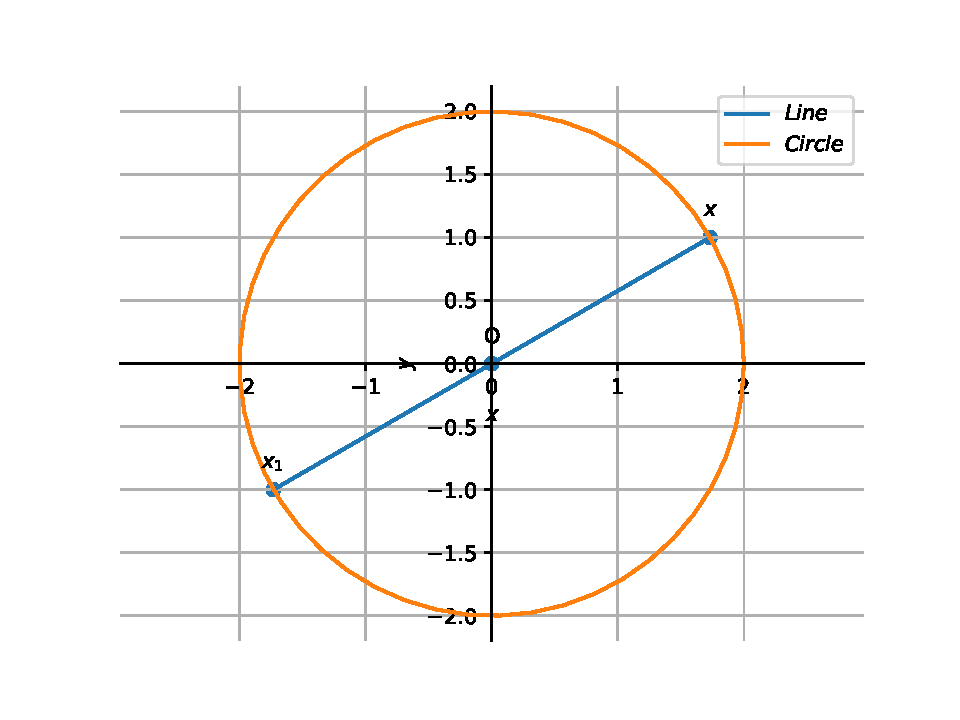
\includegraphics[width=0.75\columnwidth]{chapters/12/8/1/6/figs/conics-fig.pdf} 
		\caption{}
		\label{fig:12/8/1/6}
  	\end{figure}
  From the given information, the parameters of the  circle and line are
                      \begin{align}
			      f= -4, \vec{u}=\vec{0}, \vec{V}=\vec{I}, \vec{m}=\myvec{1 \\ \sqrt{3}}, \vec{h} = \vec{0}
		\label{eq:12/8/1/6}
                    \end{align}                                                                              
Substituting		    the above parameters in  
\eqref{eq:tangent_roots},
	  \begin{align}                                                                               
		  \mu= \sqrt{3}
	  \end{align}
	  yielding  
the desired point of intersection as                                               
\begin{align}
	\vec{x} = \myvec{\sqrt{3} \\ 1}                               
\end{align}
Note that we have chosen only the point of intersection in the first quadrant as shown in 
		\figref{fig:12/8/1/6}.
From
		\eqref{eq:12/8/1/6},
		the angle between the given line and the x axis is
\begin{align}
	\theta=30\degree
\end{align} 
and
the area of the sector is 
\begin{align}
	{\frac{\theta}{360}}\pi r^2=
	\frac{\pi}{3}
\end{align}

\item 
	Find the area of the smaller part of the circle $x^2+y^2=a^2 $ cut off by the line $x=\frac{a}{\sqrt{2}}$.
	\\
	\solution
\label{chapters/12/8/1/7}
	\begin{figure}[H]
		\centering
 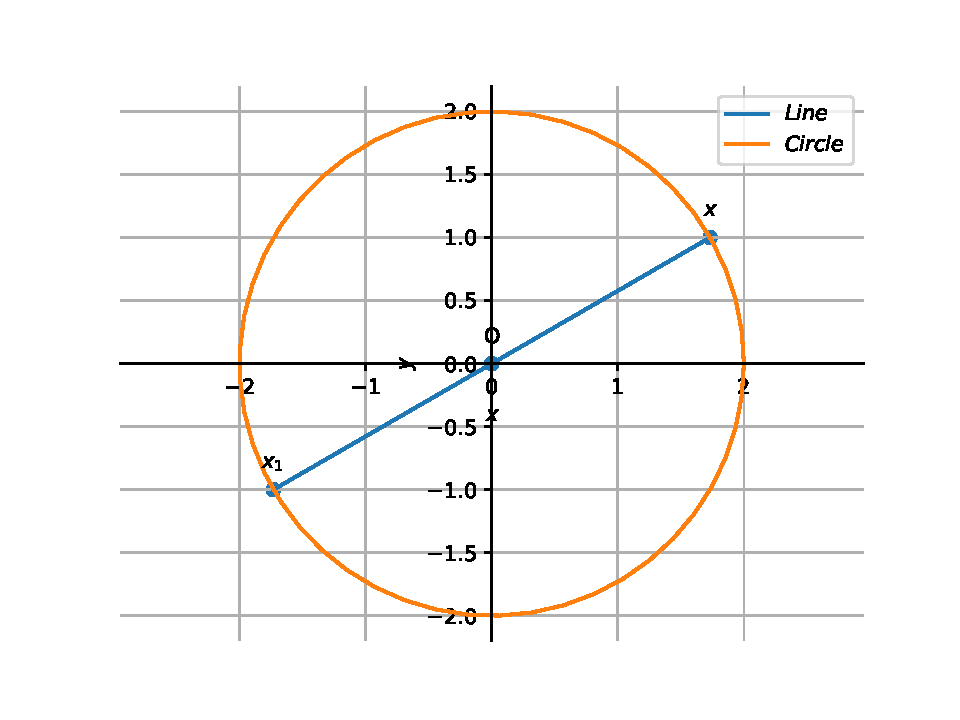
\includegraphics[width=0.75\columnwidth]{chapters/12/8/1/6/figs/conics-fig.pdf} 
		\caption{}
		\label{fig:12/8/1/6}
  	\end{figure}
  From the given information, the parameters of the  circle and line are
                      \begin{align}
			      f= -4, \vec{u}=\vec{0}, \vec{V}=\vec{I}, \vec{m}=\myvec{1 \\ \sqrt{3}}, \vec{h} = \vec{0}
		\label{eq:12/8/1/6}
                    \end{align}                                                                              
Substituting		    the above parameters in  
\eqref{eq:tangent_roots},
	  \begin{align}                                                                               
		  \mu= \sqrt{3}
	  \end{align}
	  yielding  
the desired point of intersection as                                               
\begin{align}
	\vec{x} = \myvec{\sqrt{3} \\ 1}                               
\end{align}
Note that we have chosen only the point of intersection in the first quadrant as shown in 
		\figref{fig:12/8/1/6}.
From
		\eqref{eq:12/8/1/6},
		the angle between the given line and the x axis is
\begin{align}
	\theta=30\degree
\end{align} 
and
the area of the sector is 
\begin{align}
	{\frac{\theta}{360}}\pi r^2=
	\frac{\pi}{3}
\end{align}

\item 
The area between $x = y^2$ and $x = 4$ is divided into two equal parts by the line $x = a$, find the value of a.
\\
\solution
\label{chapters/12/8/1/8}
	\begin{figure}[H]
		\centering
 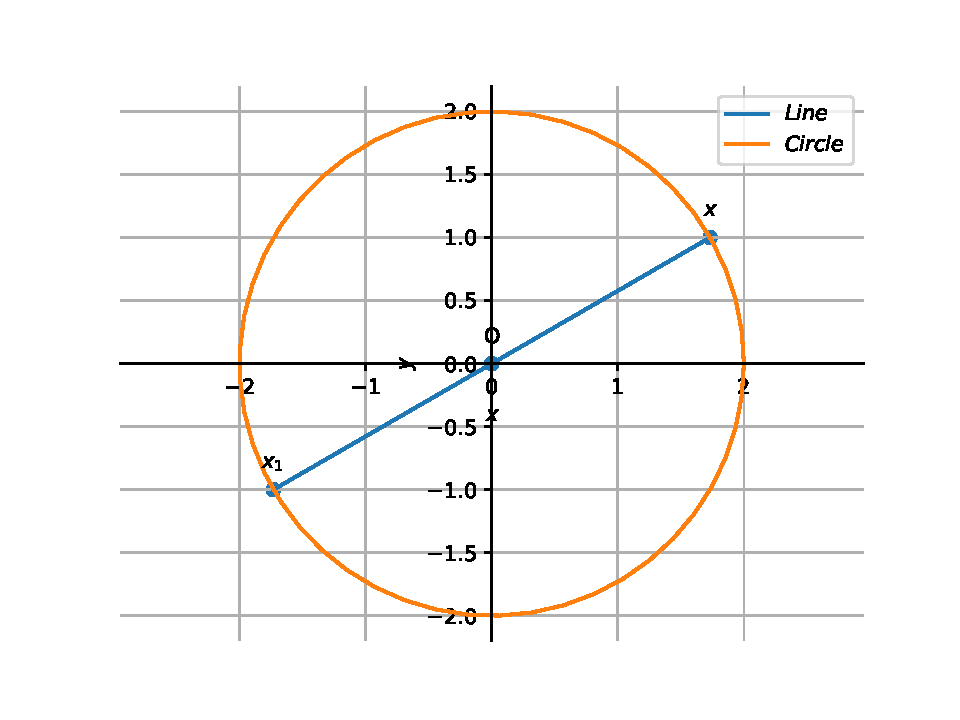
\includegraphics[width=0.75\columnwidth]{chapters/12/8/1/6/figs/conics-fig.pdf} 
		\caption{}
		\label{fig:12/8/1/6}
  	\end{figure}
  From the given information, the parameters of the  circle and line are
                      \begin{align}
			      f= -4, \vec{u}=\vec{0}, \vec{V}=\vec{I}, \vec{m}=\myvec{1 \\ \sqrt{3}}, \vec{h} = \vec{0}
		\label{eq:12/8/1/6}
                    \end{align}                                                                              
Substituting		    the above parameters in  
\eqref{eq:tangent_roots},
	  \begin{align}                                                                               
		  \mu= \sqrt{3}
	  \end{align}
	  yielding  
the desired point of intersection as                                               
\begin{align}
	\vec{x} = \myvec{\sqrt{3} \\ 1}                               
\end{align}
Note that we have chosen only the point of intersection in the first quadrant as shown in 
		\figref{fig:12/8/1/6}.
From
		\eqref{eq:12/8/1/6},
		the angle between the given line and the x axis is
\begin{align}
	\theta=30\degree
\end{align} 
and
the area of the sector is 
\begin{align}
	{\frac{\theta}{360}}\pi r^2=
	\frac{\pi}{3}
\end{align}

\item 
	Find the area of the region bounded by the parabola $y=x^2$ and $y= \abs{x}$.
\label{chapters/12/8/1/9}
\item 
Find the area bounded by the curve $x^2=4y$ and the line $x=4y-2$.
\\
\solution 
\label{chapters/12/8/1/10}
	\begin{figure}[H]
		\centering
 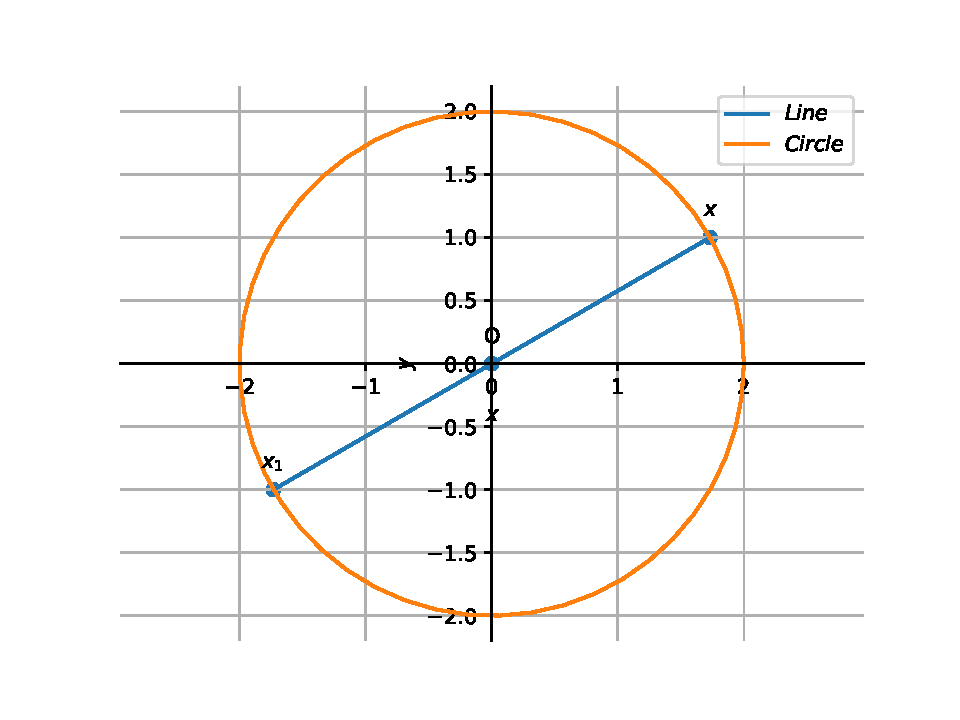
\includegraphics[width=0.75\columnwidth]{chapters/12/8/1/6/figs/conics-fig.pdf} 
		\caption{}
		\label{fig:12/8/1/6}
  	\end{figure}
  From the given information, the parameters of the  circle and line are
                      \begin{align}
			      f= -4, \vec{u}=\vec{0}, \vec{V}=\vec{I}, \vec{m}=\myvec{1 \\ \sqrt{3}}, \vec{h} = \vec{0}
		\label{eq:12/8/1/6}
                    \end{align}                                                                              
Substituting		    the above parameters in  
\eqref{eq:tangent_roots},
	  \begin{align}                                                                               
		  \mu= \sqrt{3}
	  \end{align}
	  yielding  
the desired point of intersection as                                               
\begin{align}
	\vec{x} = \myvec{\sqrt{3} \\ 1}                               
\end{align}
Note that we have chosen only the point of intersection in the first quadrant as shown in 
		\figref{fig:12/8/1/6}.
From
		\eqref{eq:12/8/1/6},
		the angle between the given line and the x axis is
\begin{align}
	\theta=30\degree
\end{align} 
and
the area of the sector is 
\begin{align}
	{\frac{\theta}{360}}\pi r^2=
	\frac{\pi}{3}
\end{align}

\item Find the area of the region bounded by the curve ${y}^2
= 4{x}$ and the line ${x} = 3$.
\label{chapters/12/8/1/11}
\item Area lying in the first quadrant and bounded by the circle ${x}^2 + {y}^2 = 4$ and the lines ${x} = 0$ and ${x} = 2$ is 
\label{chapters/12/8/1/12}
\begin{enumerate}[itemsep=+2mm]
\item $\pi$
\item $\dfrac{\pi}{2}$
\item $\dfrac{\pi}{3}$  
\item $\dfrac{\pi}{4}$
\end{enumerate}
\item Find the area of the region bounded by the curve $y^2 = 4x$, y-axis and the line $y = 3$. 
\label{chapters/12/8/1/13}
\\
\solution
\begin{enumerate}[label=\thesubsection.\arabic*, ref=\thesubsection.\theenumi]
\item Find the coordinates of the point where the line $\frac{x-1}{3} = \frac{y+4}{7} = \frac{z+4}{2}$ cuts the $XY$ plane.

\hfill (12, 2020)
    \item Find the coordinates of the point where the line through $(3, 4, 1)$ crosses the $ZX$ plane.
    \hfill (12, 2023)
	\item Find the equation of the line passing through $(2, -1, 2)$ and $(5, 3, 4)$ and the equation of the plane passing through $(2, 0, 3)$, $(1, 1, 5)$, and $(3, 2, 4)$. Also, find their point of intersection. \hfill (12, 2019)
	
	\item Find the equation of the plane which contains the line of intersection of the planes $\overrightarrow{r} \cdot (\hat{i} + 2\hat{j} + 3\hat{k}) - 4 = 0$ and $\overrightarrow{r} \cdot (2\hat{i} + \hat{j} - \hat{k}) + 5 = 0$, and which is perpendicular to the plane $\overrightarrow{r} \cdot (5\hat{i} + 3\hat{j} - 6\hat{k}) + 8 = 0$. \hfill (12, 2019)
	\item Find the equation of the plane passing through the points $(2, 5, -3)$, $(-2, -3, 5)$, and $(5, 3, -3)$. Also, find the point of intersection of this plane with the line passing through points $(3, 1, 5)$ and $(-1, -3, -1)$. \hfill (12, 2019)
	\item Find the equation of the plane passing through the intersection of the planes $\overrightarrow{r} \cdot (\hat{i} + \hat{j} + \hat{k}) = 1$ and $\overrightarrow{r} \cdot (2\hat{i} + 3\hat{j} - \hat{k}) + 4 = 0$ and parallel to the $X$ axis. Hence, find the distance of the plane from the $X$ axis. \hfill (12, 2019)
	\item Find the equation of the planes passing through the intersection of the planes $\overrightarrow{r} \cdot (3\hat{i} + 6\hat{j}) + 12 = 0$ and $\overrightarrow{r} \cdot (3\hat{i} - \hat{j} + 4\hat{k}) = 0$ and are at a unit distance from the origin.

		\hfill (12, 2019)
	\item Find the coordinates of the point where the line $\frac{x+2}{1} = \frac{y-5}{3} = \frac{z+1}{5}$ cuts the $YZ$ plane.

		\hfill (12, 2019)
	\item Find the area of the triangle $\triangle ABC$ bounded by the lines
	$4x - y + 5 = 0, 
	x + y - 5 = 0$ and 
	$x - 4y + 5 = 0$.
 \hfill (12, 2019)
\item Point $\vec{A}$ lies on the line segment $XY$ joining $\vec{X}(6, -6)$ and $\vec{Y}(-4, -1)$ in such a way that $\frac{XA}{XY} = \frac{2}{5}$. If point $\vec{A}$ also lies on the line $3x + k(y + 1) = 0$, find the value of $k$.

	\hfill (10, 2019)
\item Find the ratio in which the line $x - 3y = 0$ divides the line segment joining the points $(-2, -5)$ and $(6, 3)$. Find the coordinates of the point of intersection. \hfill (10, 2019)
\item Find the distance of the point $(-1, -5, -10)$ from the point of intersection of the line 
	$\overrightarrow{r} = 2\hat{i} - \hat{j} + 2\hat{k} + \lambda \brak{3\hat{i} + 4\hat{j} + 2\hat{k}}$ 
and the plane 
		$\overrightarrow{r} \cdot \brak{\hat{i} - \hat{j} + \hat{k}} = 5.$
\hfill (12, 2018)
\item Find the equation of the plane passing through the points $(2, 5, -3)$, $(-2, -3, 5)$, and $(5, 3, -3)$. Also, find the point of intersection of this plane with the line passing through points $(3, 1, 5)$ and $(-1, -3, -1)$. \hfill (12, 2018)
\item Find the value of $\lambda$ for which the lines 
$\frac{x - 5}{5\lambda + 2} = \frac{2 - y}{5} = \frac{1 - z}{-1}$
and
$\frac{x}{1} = \frac{y + \frac{1}{2}}{2\lambda} = \frac{z - 1}{3}$
are perpendicular to each other.
Hence, find whether the lines intersect or not.

		\hfill (12, 2018)
\item Find the equation of the plane which contains the line of intersection of the planes $ \overrightarrow{r}.\brak{\hat{i} + 2\hat{j}+3\hat{k}}-4=0$ , $\overrightarrow{r}.\brak{2\hat{i} + \hat{j} - \hat{k}}+5=0$ and which is perpendicular to the plane $\overrightarrow{r}.\brak{5\hat{i} + 3\hat{j} - 6\hat{k}}+8=0$.
\hfill (12, 2018)
\item Find the equation of planes passing through the intersection  of the planes $\overrightarrow{r} \cdot \brak{2\hat{i}+6\hat{j}}+12=0$ and $\overrightarrow{r} \cdot \brak{3\hat{i}-\hat{j}+4\hat{k}}=0$ and are at a unit distance from origin.

\hfill (12, 2018) 
\item Find the value of $\lambda$, so that the lines $\frac{1-x}{3}=\frac{7y-14}{\lambda}=\frac{z-3}{2}$ and $\frac{7-7x}{3\lambda}=\frac{y-5}{1}=\frac{6-z}{5}$ are at right angles. Also, find whether the lines are intersecting or not.       
\hfill (12, 2018) 
\item Find the equation of the plane which contains the line of intersection of the planes
          $\overrightarrow{r}.\myvec{\hat{i} - 2\hat{j} + 3\hat{k}} - 4  = 0$ 
	  and
          $\overrightarrow{r}.\myvec{-2\hat{i} + \hat{j} + \hat{k}} + 5  = 0$
      and whose intercept on $X$ axis is equal to that of on $Y$ axis. \hfill (12, 2016)
\item Find the coordinates of the point where the line through the points $\vec{P}\brak{4, 3, 2}$ and $\vec{Q}\brak{5,1,6}$ crosses the $XZ$ plane. Also find the angle which this line makes with the $XZ$ plane. \hfill (12, 2016)
\item Find the coordinates of the point where the line through the points $\vec{A}\brak{3,4,1}$ and $\vec{B}\brak{5,1,6}$ crosses the $XZ$ plane. Also find the angle which this line makes with the $XZ$ plane. \hfill (12, 2016)
\item Find the equation of the plane passing through the line of intersection of planes 
$\vec{r}\cdot\brak{2\overrightarrow{i}+2\overrightarrow{j}-3\overrightarrow{k}}=7$, $\vec{r}\cdot\brak{2\overrightarrow{i}+5\overrightarrow{j}+3\overrightarrow{k}}=9$
such that the intercepts made by the plane on $X$ axis and $Z$ axis are equal. \hfill (12, 2015)
\item Find the equations of the diagonals of the parallelogram $PQRS$ whose vertices are $\vec{P}(4,2,-6)$, $\vec{Q}(5,-3,1)$, $\vec{R}(12,4,5)$ and $\vec{S}(11,9,-2)$. Use these equations to find the point of intersection of diagonals. \hfill (12, 2023)
\item Find the co-ordinates of the point where the line $\frac{x-3}{-1}=\frac{y+4}{1}=\frac{z+5}{6}$ crosses the plane passing through the points $\left(\frac{7}{2},0,0\right),(0,7,0),(0,0,7)$. \hfill (12, 2022)

\item Find the equation of the plane through the line of intersection of the planes
		$\vec{r}\cdot(\hat{i}+3\hat{j})+6=0$,
		$\vec{r}\cdot(3\hat{i}-\hat{j}-4\hat{k})=0$
	which is at a unit distance from the origin.

	\hfill (12, 2022)
\item Find the distance of the point $(1,-2, 9)$ from the point of intersection of the line
		$\vec{r}=4\hat{i}+2\hat{j}+7\hat{k}+\lambda(3\hat{i}+4\hat{j}+2\hat{k})$
	and the plane
		$\vec{r}\cdot(\hat{i}-\hat{j}+\hat{k})=10$.
\hfill (12, 2022)

\item Find the area bounded by the curves $y=\abs{x-1}$ and $y=1$. \hfill (12, 2022)

\item Find the coordinates of the point where the line through $(4,-3,-4)$ and $(3,-2,2)$ crosses the plane $2x+y+z=6$. \hfill (12, 2022)
\item Find the equation of the plane through the line of intersection of the planes 
  $\vec{r} \cdot \brak{i+3j} + 6 = 0 $
  and
  $\vec{r} \cdot \brak{3i - j - 4k} = 0$,
which is at a unit distance from the origin.

\hfill (12, 2021)
\item Find the area of the region bounded by the lines $3x - 2y + 1 = 0, 2x + 3y - 21 = 0$ and $x - 5y + 9 = 0$. \hfill (12, 2019)
\item Draw the graph of the equations $x - y + 1 = 0$ and $3x + 2y - 12 = 0$. Using this graph, find the values of $x$ and $y$ which satisfy both the equations.
\hfill (10, 2021)

\item Find the area of the region bounded by the line $y = 3x + 2,$ the $X$ axis and the ordinates $x = - 2$ and $x = 1$. \hfill (12, 2019)
\item Find the equation of the line passing through $\brak{2,-1, 2}$ and $\brak{5, 3, 4}$ and of the plane passing through $\brak{2, 0, 3}$, $\brak{1, 1, 5}$ and $\brak{3, 2, 4}$. Also, find their point of intersection.

	\hfill (12, 2018)
\item Find the length of the intercept, cut off by the plane $2x+y-z=5$ on the $X$ axis.

	\hfill (12, 2018)
\item Find the area of the region bounded by the lines $3x-2y+1$=$0$, $2x+3y-21$ = $0$ , and  $x-5y+9$ = $0$. \hfill (12, 2018)
\item Find the area of the region bounded by the line $y = 3x + 2$, the $X$ axis and the ordinates and the ordinates $x=-2$ and $x=1$. \hfill (12, 2018)
\item Find the coordinates of the point where the line through the points $\brak{3, – 4, – 5}$ and $\brak{2, – 3, 1}$, crosses the plane determined by the points $\brak{1, 2, 3}, \brak{4, 2, – 3}$ and $\brak{0, 4, 3}$.

	\hfill (12, 2017)
\item Show that the lines $\frac{x-1}{3} = \frac{y-1}{-1} = \frac{z+1}{0} $ and $\frac{x-4}{2} = \frac{y}{0} = \frac{z+1}{3} $ intersect. Find their point of intersection. \hfill (12, 2016)
	\item Find the area of the triangular region whose sides have the equations $y = 2x + 1$, $y = 3x + 1$, and $x = 4$. \hfill (12, 2019)
\item Find the area of the region bounded by the lines $3x - 2y + 1 = 0, 2x + 3y - 21 = 0$ and $x - 5y + 9 = 0$.
\hfill (12, 2019)
\item Find the area of the region bounded by the line
$y = 3x + 2,$ the $X$ axis and the ordinates $x = - 2$ and $x = 1$.
\hfill (12, 2019)
\end{enumerate}

\item 
Find the area of the region bounded by the curve $x^2=4y$ and the lines $y=2$ and $y=4$ and the y-axis in the first quadrant.
\\
\solution
\label{chapters/12/8/3/3}
	\begin{figure}[H]
		\centering
 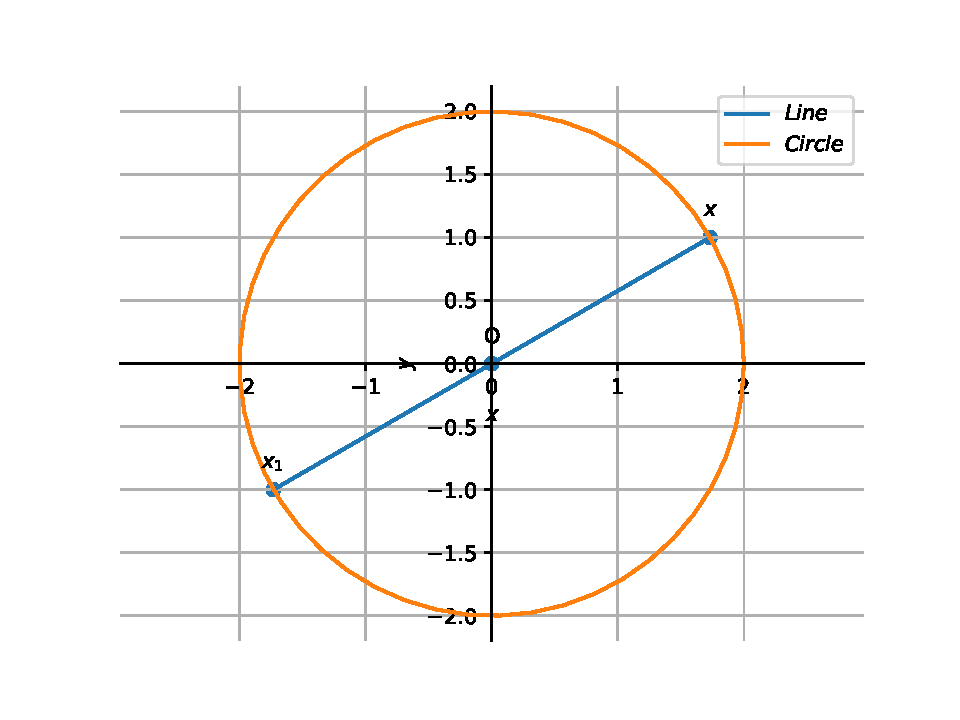
\includegraphics[width=0.75\columnwidth]{chapters/12/8/1/6/figs/conics-fig.pdf} 
		\caption{}
		\label{fig:12/8/1/6}
  	\end{figure}
  From the given information, the parameters of the  circle and line are
                      \begin{align}
			      f= -4, \vec{u}=\vec{0}, \vec{V}=\vec{I}, \vec{m}=\myvec{1 \\ \sqrt{3}}, \vec{h} = \vec{0}
		\label{eq:12/8/1/6}
                    \end{align}                                                                              
Substituting		    the above parameters in  
\eqref{eq:tangent_roots},
	  \begin{align}                                                                               
		  \mu= \sqrt{3}
	  \end{align}
	  yielding  
the desired point of intersection as                                               
\begin{align}
	\vec{x} = \myvec{\sqrt{3} \\ 1}                               
\end{align}
Note that we have chosen only the point of intersection in the first quadrant as shown in 
		\figref{fig:12/8/1/6}.
From
		\eqref{eq:12/8/1/6},
		the angle between the given line and the x axis is
\begin{align}
	\theta=30\degree
\end{align} 
and
the area of the sector is 
\begin{align}
	{\frac{\theta}{360}}\pi r^2=
	\frac{\pi}{3}
\end{align}

\item 
	Find the area enclosed by the parabola $4y=3x^2 $ and the line $2y=3x+12$.\\
	\solution
\label{chapters/12/8/3/7}
	\begin{figure}[H]
		\centering
 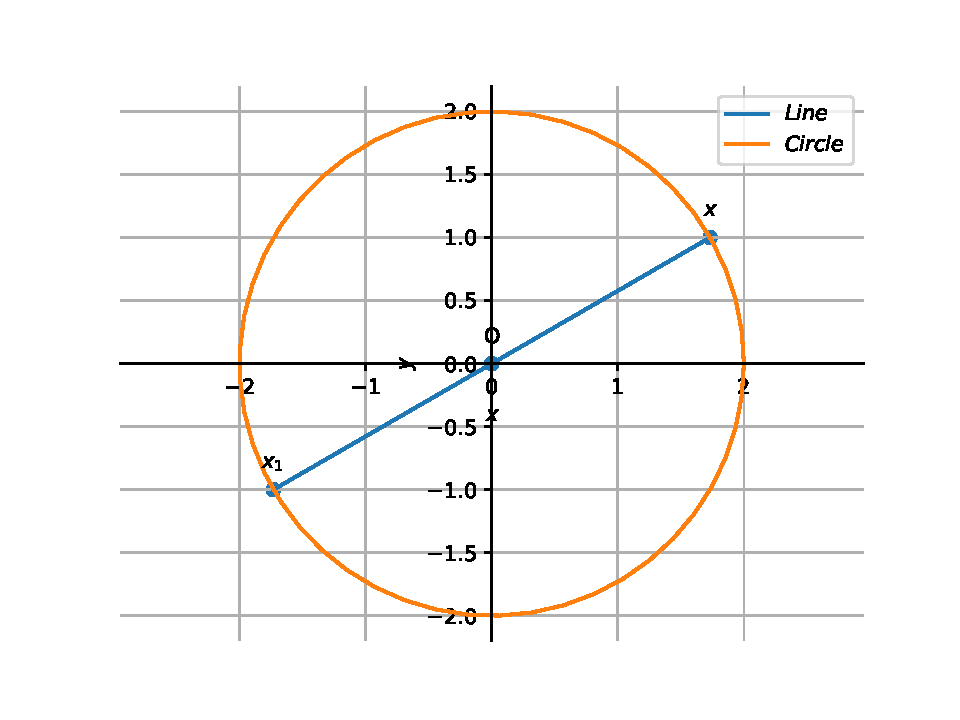
\includegraphics[width=0.75\columnwidth]{chapters/12/8/1/6/figs/conics-fig.pdf} 
		\caption{}
		\label{fig:12/8/1/6}
  	\end{figure}
  From the given information, the parameters of the  circle and line are
                      \begin{align}
			      f= -4, \vec{u}=\vec{0}, \vec{V}=\vec{I}, \vec{m}=\myvec{1 \\ \sqrt{3}}, \vec{h} = \vec{0}
		\label{eq:12/8/1/6}
                    \end{align}                                                                              
Substituting		    the above parameters in  
\eqref{eq:tangent_roots},
	  \begin{align}                                                                               
		  \mu= \sqrt{3}
	  \end{align}
	  yielding  
the desired point of intersection as                                               
\begin{align}
	\vec{x} = \myvec{\sqrt{3} \\ 1}                               
\end{align}
Note that we have chosen only the point of intersection in the first quadrant as shown in 
		\figref{fig:12/8/1/6}.
From
		\eqref{eq:12/8/1/6},
		the angle between the given line and the x axis is
\begin{align}
	\theta=30\degree
\end{align} 
and
the area of the sector is 
\begin{align}
	{\frac{\theta}{360}}\pi r^2=
	\frac{\pi}{3}
\end{align}

\item 
	Find the area of the smaller region bounded by the ellipse $\frac{x^2}{9}+\frac{y^2}{4}=1$
and the line $\frac{x}{3}+\frac{y}{2}=1$.\\
\solution
\label{chapters/12/8/3/8}
	\begin{figure}[H]
		\centering
 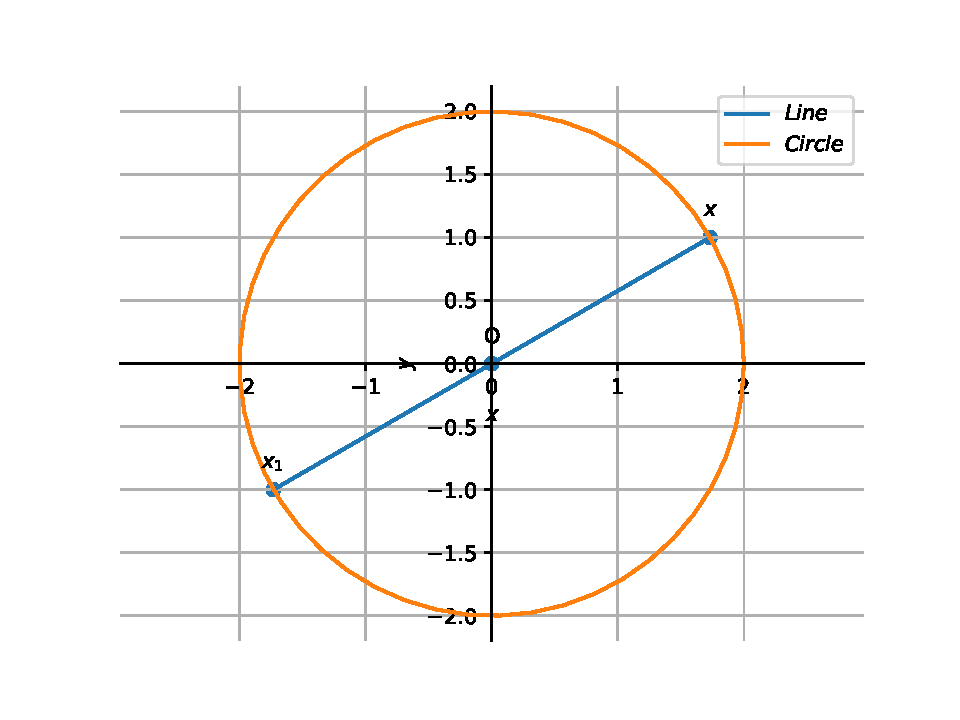
\includegraphics[width=0.75\columnwidth]{chapters/12/8/1/6/figs/conics-fig.pdf} 
		\caption{}
		\label{fig:12/8/1/6}
  	\end{figure}
  From the given information, the parameters of the  circle and line are
                      \begin{align}
			      f= -4, \vec{u}=\vec{0}, \vec{V}=\vec{I}, \vec{m}=\myvec{1 \\ \sqrt{3}}, \vec{h} = \vec{0}
		\label{eq:12/8/1/6}
                    \end{align}                                                                              
Substituting		    the above parameters in  
\eqref{eq:tangent_roots},
	  \begin{align}                                                                               
		  \mu= \sqrt{3}
	  \end{align}
	  yielding  
the desired point of intersection as                                               
\begin{align}
	\vec{x} = \myvec{\sqrt{3} \\ 1}                               
\end{align}
Note that we have chosen only the point of intersection in the first quadrant as shown in 
		\figref{fig:12/8/1/6}.
From
		\eqref{eq:12/8/1/6},
		the angle between the given line and the x axis is
\begin{align}
	\theta=30\degree
\end{align} 
and
the area of the sector is 
\begin{align}
	{\frac{\theta}{360}}\pi r^2=
	\frac{\pi}{3}
\end{align}

\item 
Find the area of the region bounded by the curve $x^2=y$ and the lines $y=x+2$ and the $x$ axis.
\label{chapters/12/8/3/10}
\item 
Find   the area bounded by the curve $y=x|x|, x$-axis and the ordinates $x$=-1 and $x$=1.
\label{chapters/12/8/3/17}
\item 
	Find the area of the region bounded by the curves $y=x^2+2$, $y=x$, $x=0$ and $x=3. $
\label{chapters/12/8/2/3}
\item 
Find the smaller area enclosed by the circle $x^2 + y^2 = 4$ and the line $x + y = 2$. 
\\
\solution
\label{chapters/12/8/2/6}
	\begin{figure}[H]
		\centering
 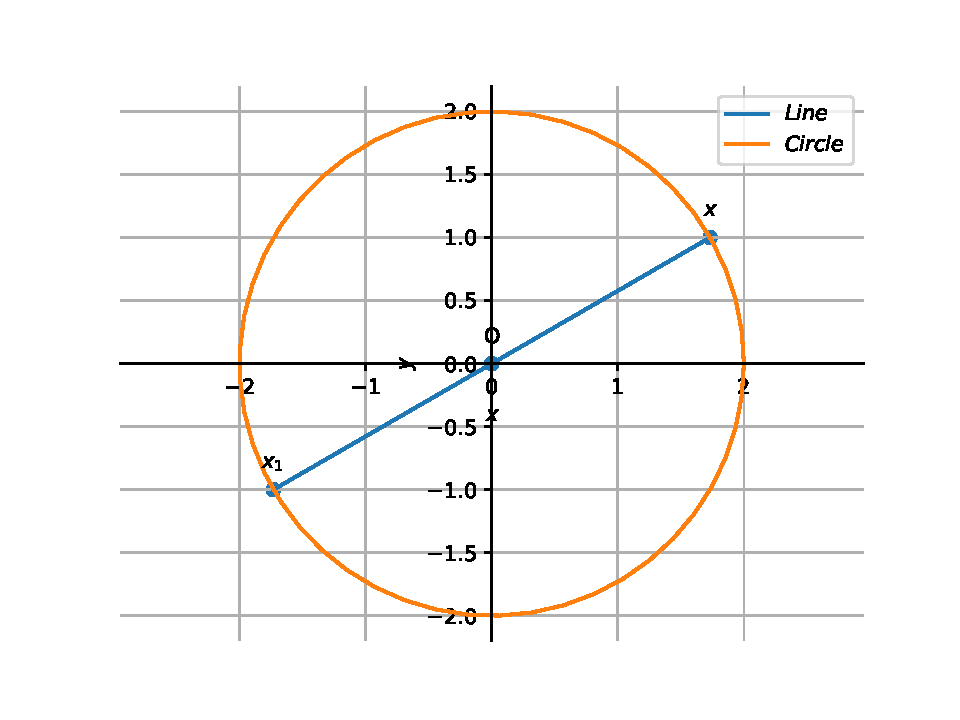
\includegraphics[width=0.75\columnwidth]{chapters/12/8/1/6/figs/conics-fig.pdf} 
		\caption{}
		\label{fig:12/8/1/6}
  	\end{figure}
  From the given information, the parameters of the  circle and line are
                      \begin{align}
			      f= -4, \vec{u}=\vec{0}, \vec{V}=\vec{I}, \vec{m}=\myvec{1 \\ \sqrt{3}}, \vec{h} = \vec{0}
		\label{eq:12/8/1/6}
                    \end{align}                                                                              
Substituting		    the above parameters in  
\eqref{eq:tangent_roots},
	  \begin{align}                                                                               
		  \mu= \sqrt{3}
	  \end{align}
	  yielding  
the desired point of intersection as                                               
\begin{align}
	\vec{x} = \myvec{\sqrt{3} \\ 1}                               
\end{align}
Note that we have chosen only the point of intersection in the first quadrant as shown in 
		\figref{fig:12/8/1/6}.
From
		\eqref{eq:12/8/1/6},
		the angle between the given line and the x axis is
\begin{align}
	\theta=30\degree
\end{align} 
and
the area of the sector is 
\begin{align}
	{\frac{\theta}{360}}\pi r^2=
	\frac{\pi}{3}
\end{align}

\item Find the area of the region bounded by the curves $y^2 = 9x$, $y = 3x$.
\item Find the area of the region bounded by the parabola $y^2 = 2px$, $x^2 = 2py$.
\item Find the area of the region bounded by the curve $y = x^2\text{ and }y = x + 6\text{ and }x = 0$.
\item Find the area of the region bounded by the curve $y^2 = 4x$, $x^2 = 4y$.
\item Find the area of the region included between $y^2 = 9x\text{ and }y =x$
\item Find the area of the region enclosed by the parabola $x^2 = y$ and the line $y = x + 2$
\item Find the area of region bounded by the line $x = 2$ and the parabola $y^2 = 8x$
\item Sketch the region ${(x,0) : y = \sqrt{4 - x^2}}$ and $x$-axis. Find the area of the region using integration.
\item Calculate the area under the curve $y = 2\sqrt{x}$ included between the lines $x = 0\text{ and }x = 1$.
\item Using integration, find the area of the region bounded by the line $2y = 5x + 7$, $x$-axis and the lines $x = 2\text{ and }x =8$.
\item Draw a rough sketch of the curve $y = \sqrt{x - 1}$ in the interval $[1, 5]$. Find the area under the curve and between the lines $x = 1\text{ and }x = 5$.
\item Determine the area under the curve $y = \sqrt{a^2 - x^2}$ included between the lines $x = 0\text{ and }x = a$
\item Find the area of the region bounded by $y = \sqrt{x}\text{ and }y = x$.
\item Find the area enclosed by the curve $y = - x^2$ and the straight line $x + y + 2 = 0$.
\item Find the area bounded by the curve $y = \sqrt{x}$, $x = 2y + 3$ in the first quadrant and $x$-axis.
\item Draw a rough sketch of the region ${(x, y) : y^2 \lessgtr 6ax\text{ and }x^2 + y^2 \lessgtr 16a^2}$.
\item Draw a  rough sketch of the given curve $y =1 + \abs{x + 1}$, $x = -3$, $x = 3$, $y = 0$, and find the area of the region bounded by them, using integration.
\item The area of the region bounded by the curve $x^2 = 4y$ and the straight line $x = 4y - 2$ is
\begin{enumerate}
\item $\frac{3}{8}$ sq units 
\item $\frac{5}{8}$ sq units
\item $\frac{7}{8}$ sq units 
\item $\frac{9}{8}$ sq units
\end{enumerate}
\item The area of the region bounded by the curve $y = \sqrt{16 - x^2}$ and $x$-axis is 
\begin{enumerate}
\item 8 sq units 
\item ${20\pi}$ sq units
\item ${16\pi}$ sq units
\item ${256\pi}$ sq units
\end{enumerate}
\item Area of the region in the first quadrant enclosed by the $x$-axis, the line $y = x$ and the circle $x^2 + y^2 = 32$ is 
\begin{enumerate}
\item ${16\pi}$ sq units 
\item ${4\pi}$ sq units
\item ${32\pi}$ sq units
\item ${24\pi}$ sq units
\end{enumerate}
\item The area of the region bounded by parabola $y^2 = x$ and the straight line $2y = x$ is
\begin{enumerate}
\item $\frac{4}{3}$ sq units
\item 1 sq units
\item $\frac{2}{3}$ sq units 
\item $\frac{1}{3}$ sq units
\end{enumerate}
\item Find the equation of a circle whose centre is (3,1) and which cuts off a chord of length  6 units on the  line $2x-5y+18=0$.
\end{enumerate}
